% Datasheet skAInet Edge-Compute v1.5 (English)
\documentclass[10pt,a4paper]{article}
\usepackage[margin=20mm,top=18mm,bottom=20mm]{geometry}
\usepackage[T1]{fontenc}
\usepackage[utf8]{inputenc}
\usepackage[english]{babel}
\usepackage{helvet}\renewcommand{\familydefault}{\sfdefault}
\usepackage{booktabs,array,tabularx,siunitx,microtype}
\usepackage{tikz}
\usetikzlibrary{calc,arrows.meta}
\usepackage{xcolor}
\usepackage{graphicx}
\definecolor{skred}{HTML}{C8102E}
\definecolor{skgray}{HTML}{444444}
\usepackage{fancyhdr}
\pagestyle{fancy}\fancyhf{}
\fancyhead[L]{\small\textbf{skAInet Edge-Compute v1.5} — Datasheet}
\fancyhead[R]{\small Auto-Intern GmbH, Bochum, Germany}
\fancyfoot[L]{\small DS-EC-1.5 · September 2026}
\fancyfoot[R]{\small Page \thepage}
\renewcommand{\headrulewidth}{0.4pt}
\setlength{\parindent}{0pt}
\sisetup{per-mode=symbol}

% dimensioning styles
\tikzset{
  dimline/.style={<->, >=Latex, line width=0.4pt, draw=skgray},
  extline/.style={line width=0.3pt, draw=skgray},
  dimtext/.style={fill=white, inner sep=1pt, font=\footnotesize, text=black},
  part/.style={line width=0.8pt, draw=black},
  hidden/.style={line width=0.4pt, draw=skgray, dash pattern=on 2pt off 1.5pt},
  center/.style={line width=0.3pt, draw=skgray, dash pattern=on 6pt off 1.5pt on 1pt off 1.5pt},
}

\begin{document}

%=====================================================================
% Page 1 — Overview & specification
%=====================================================================
\begin{minipage}[b]{0.66\textwidth}
{\LARGE\textbf{\textcolor{skred}{skAInet} Edge-Compute}}\quad{\Large v1.5}

\vspace{2mm}
{\large Programmable M12-PoE switch, router, and Linux compute module for industrial edge data acquisition}
\end{minipage}\hfill
\begin{minipage}[b]{0.26\textwidth}
\raggedleft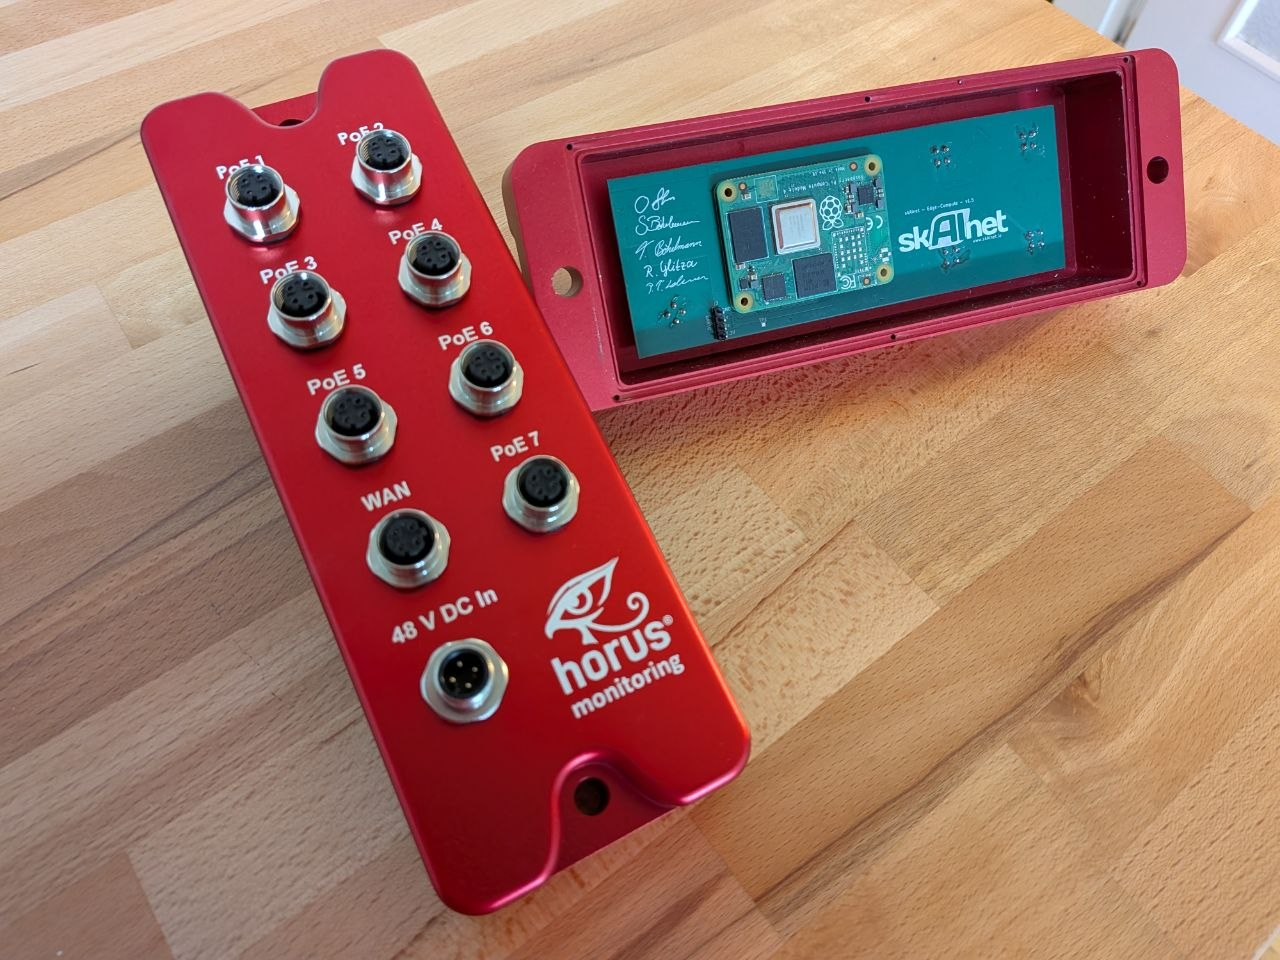
\includegraphics[width=\textwidth]{edge-branded.jpg}
\end{minipage}

\vspace{2mm}\hrule\vspace{2mm}

\textbf{Description.} The skAInet Edge-Compute is Auto-Intern GmbH's
universal data-acquisition and monitoring platform. An anodized aluminum
enclosure, machined from a single block, combines an 8-port switch with
seven external M12 PoE+ LAN ports (D-coded), a separate M12 WAN port
(D-coded), and a swappable compute module (Raspberry Pi CM
pin-compatible). All connections use sealing M12 connectors; the device
operates under water at up to \SI{1}{bar}. Measurement data is buffered,
pre-processed, and analyzed on the device; only data explicitly
configured for forwarding reaches the upstream network.

\vspace{2mm}
\begin{minipage}[t]{0.48\textwidth}
\textbf{Compute}\par\vspace{1mm}
\begin{tabularx}{\textwidth}{@{}>{\bfseries}p{2.9cm}X@{}}
\toprule
Module & Raspberry Pi CM4 (standard); CM5 or NVIDIA Jetson on request, pin-compatible, swappable \\
CPU & 8 cores, 64-bit ARM, \SI{1.5}{GHz} \\
RAM & \SI{8}{GB} LPDDR4-3200 \\
Storage & \SI{32}{GB} eMMC \\
Operating system & Yocto Linux with documented SBOM (EU Cyber Resilience Act); encrypted OTA updates or offline via USB image \\
\bottomrule
\end{tabularx}

\vspace{2mm}
\textbf{Networking}\par\vspace{1mm}
\begin{tabularx}{\textwidth}{@{}>{\bfseries}p{2.9cm}X@{}}
\toprule
WAN & 1$\times$ M12 D-coded (4-pin), Gigabit Ethernet, DHCP client \\
LAN & 7$\times$ M12 D-coded (4-pin, Ethernet) with PoE+, internally connected to an 8-port switch (DHCP server, 192.168.199.1/24) \\
PoE & IEEE~802.3at (PoE+) on all 7 LAN ports; typical devices draw up to approx.\ \SI{10}{W} \\
Cabling & 1 certified Cat-5e M12 cable per device \\
Data interface & Live data via WebSocket (port 8001, JSON, ns timestamps) \\
Upstream APIs & REST, WebSocket, webhooks, MQTT, OPC~UA, Modbus-TCP, EPICS, gRPC, AMQP, CoAP, SNMP, Prometheus, InfluxDB, SFTP/rsync \\
Capacity & 250+ concurrent channels proven in production \\
\bottomrule
\end{tabularx}
\end{minipage}\hfill
\begin{minipage}[t]{0.48\textwidth}
\textbf{Power}\par\vspace{1mm}
\begin{tabularx}{\textwidth}{@{}>{\bfseries}p{2.9cm}X@{}}
\toprule
Input & \SIrange{48}{72}{V} DC via M12 A-coded (4-pin, TE T4140012041-000) \\
PSU & recommended $\geq$ \SI{100}{W} \\
Minimum & \SI{25}{W} (compute only, no PoE loads) \\
\bottomrule
\end{tabularx}

\vspace{2mm}
\textbf{Environmental \& mechanical}\par\vspace{1mm}
\begin{tabularx}{\textwidth}{@{}>{\bfseries}p{2.9cm}X@{}}
\toprule
Enclosure & anodized aluminum, machined from solid, shockproof \\
Ingress protection & IP67, all ports and back plate sealed; operation under water up to \SI{1}{bar} \\
Temperature & \SIrange{-25}{70}{\celsius} \\
Dimensions & $216 \times 75 \times 32$ \si{mm} (W$\times$D$\times$H); overall depth incl.\ connectors approx.\ \SI{51}{mm} \\
Front plate & 8$\times$ M12 D-coded (7$\times$ PoE LAN, 1$\times$ WAN) in a 4$\times$2 grid, 1$\times$ M12 A-coded power-in; custom branding available \\
\bottomrule
\end{tabularx}

\vspace{2mm}
\textbf{Software}\par\vspace{1mm}
\begin{tabularx}{\textwidth}{@{}>{\bfseries}p{2.9cm}X@{}}
\toprule
Access & SSH (port 22022); custom applications in C++ or Python, Docker deployment; minimal examples on GitHub \\
Remote support & optional manufacturer remote maintenance via encrypted access, can be disabled \\
Updates & encrypted OTA updates via the WAN port or offline via USB image \\
\bottomrule
\end{tabularx}

\vspace{2mm}
\textbf{Field references}\par\vspace{1mm}
{\small DB Netz DIANA (switch-point motor monitoring) · Kelvion (IR fouling detection) · Kurtz Ersa / Global Point HORUS (soldering process monitoring) · RUB/GSI-FAIR PANDA (luminosity detector) · MSU CBE (river impedance spectroscopy) · NexuFed AI / RUB (federated pump monitoring)}
\end{minipage}

\vspace{2mm}\hrule\vspace{1.5mm}
{\small
\textbf{Manufacturer:} Auto-Intern GmbH · Herner Str.\ 299, Building B29, 44809 Bochum, Germany · info@auto-intern.de · +49\,234\,9345\,1121\\
\textbf{Price:} from 260\,€ / \$299 net · \textbf{Documentation:} edge-compute.skainet.io}

%=====================================================================
% Sheets 1-3 — dimensioned drawing 1:1, one view per page, module vertical
%=====================================================================
\newpage
\thispagestyle{fancy}
\begin{center}
{\large\textbf{Dimensioned Drawing — Enclosure Edge-Compute v1.5}}\\[1mm]
{\small All dimensions in mm · General tolerances ISO 2768-mK · Material: Al, anodized · \textbf{Scale 1:1} · Sheet 1/4: front view}
\end{center}
\vfill
\begin{center}
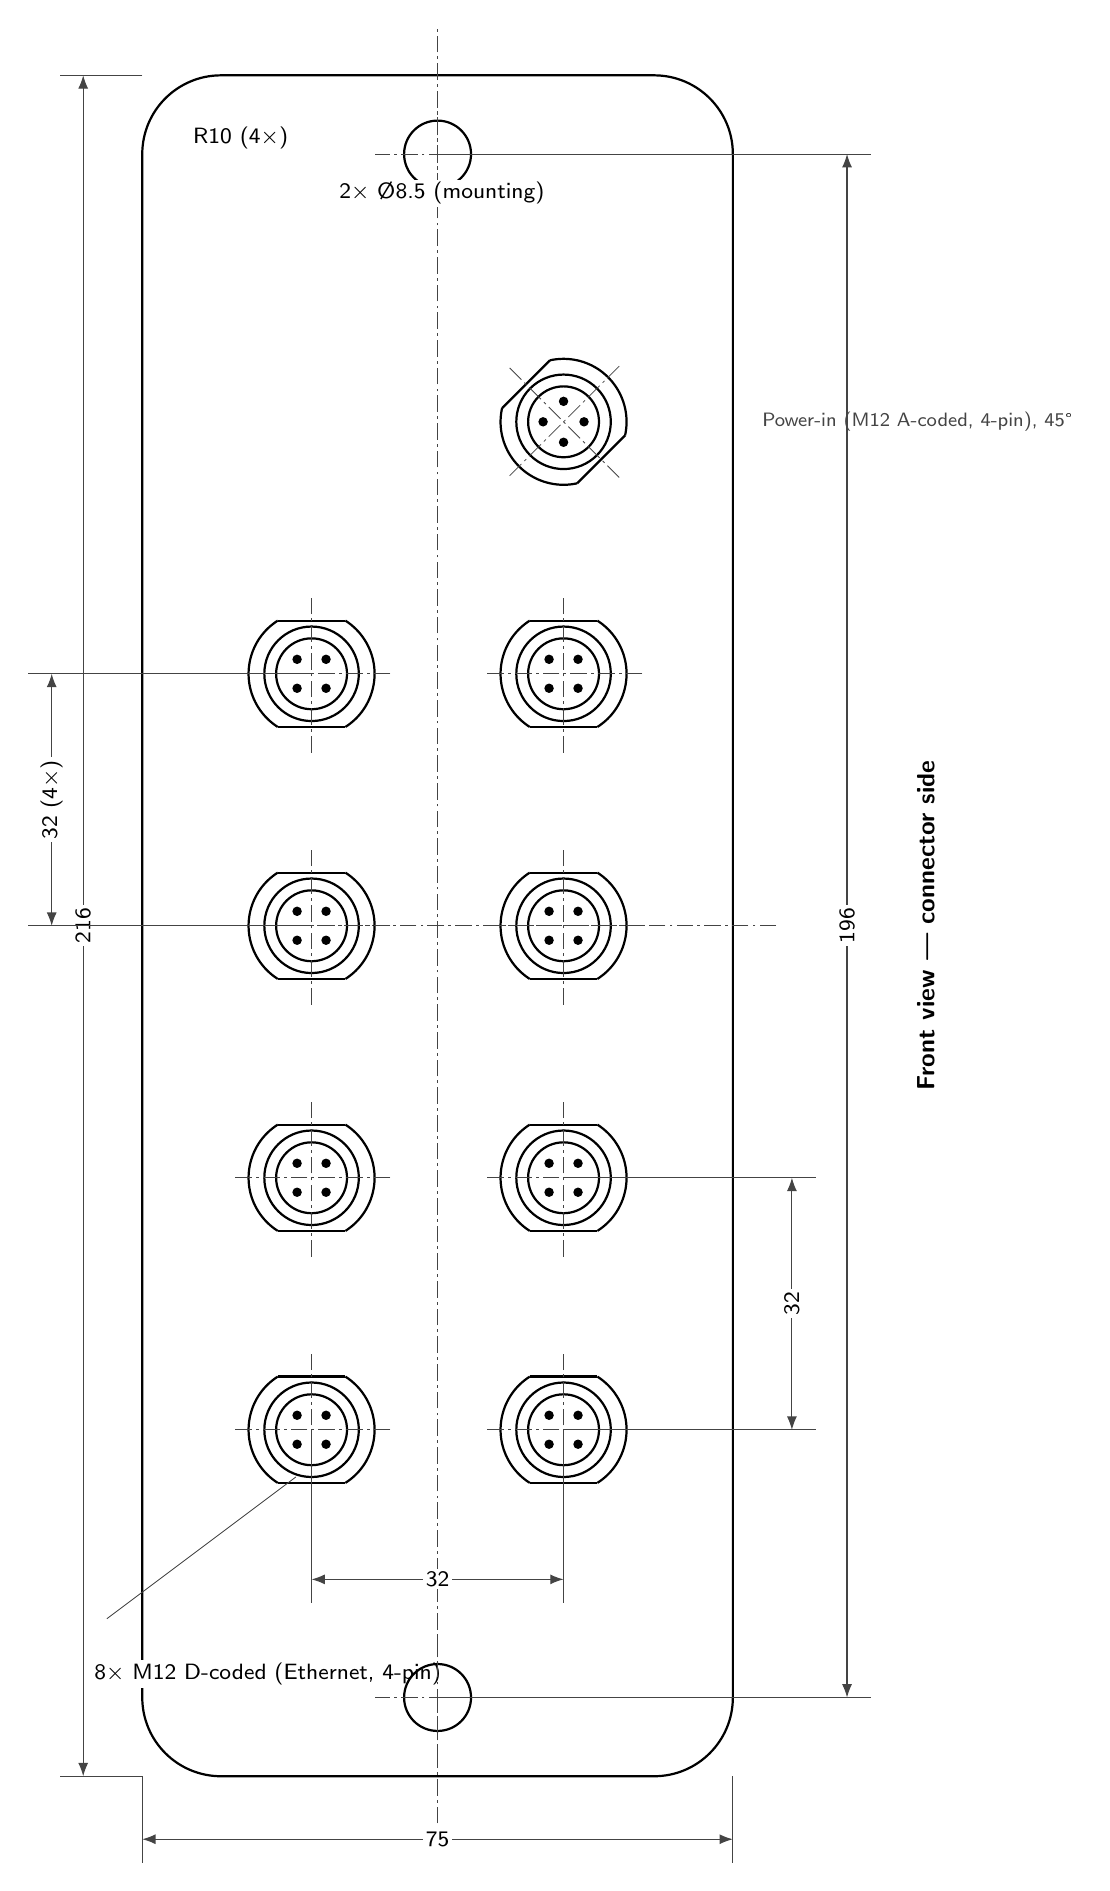
\begin{tikzpicture}[scale=0.1, rotate=90]  % 1:1, module vertical
  % outer contour 216 x 75, corner radius 10
  \draw[part, rounded corners=1cm] (-108,-37.5) rectangle (108,37.5);
  \draw[center] (-114,0) -- (114,0);
  \draw[center] (0,-43) -- (0,43);
  % M12 sockets D-coded, 4x2 grid, pitch 32/32
  \foreach \x in {-64,-32,0,32}{
    \foreach \y in {-16,16}{
      \begin{scope}[shift={(\x,\y)}]
        \draw[part] (6.75,{sqrt(64-6.75*6.75)}) arc[start angle={acos(6.75/8)}, end angle={180-acos(6.75/8)}, radius=8];
        \draw[part] (-6.75,{-sqrt(64-6.75*6.75)}) arc[start angle={180+acos(6.75/8)}, end angle={360-acos(6.75/8)}, radius=8];
        \draw[part] (6.75,{sqrt(64-6.75*6.75)}) -- (6.75,{-sqrt(64-6.75*6.75)});
        \draw[part] (-6.75,{sqrt(64-6.75*6.75)}) -- (-6.75,{-sqrt(64-6.75*6.75)});
        \draw[part] (0,0) circle[radius=6];
        \draw[part] (0,0) circle[radius=4.5];
        \foreach \a in {45,135,225,315} \fill (\a:2.6) circle[radius=0.6];
        \draw[center] (-10,0)--(10,0); \draw[center] (0,-10)--(0,10);
      \end{scope}
    }
  }
  % power socket A-coded, rotated 45°
  \begin{scope}[shift={(64,-16)}, rotate=45]
    \draw[part] (6.75,{sqrt(64-6.75*6.75)}) arc[start angle={acos(6.75/8)}, end angle={180-acos(6.75/8)}, radius=8];
    \draw[part] (-6.75,{-sqrt(64-6.75*6.75)}) arc[start angle={180+acos(6.75/8)}, end angle={360-acos(6.75/8)}, radius=8];
    \draw[part] (6.75,{sqrt(64-6.75*6.75)}) -- (6.75,{-sqrt(64-6.75*6.75)});
    \draw[part] (-6.75,{sqrt(64-6.75*6.75)}) -- (-6.75,{-sqrt(64-6.75*6.75)});
    \draw[part] (0,0) circle[radius=6];
    \draw[part] (0,0) circle[radius=4.5];
    \foreach \a in {45,135,225,315} \fill (\a:2.6) circle[radius=0.6];
    \draw[center] (-10,0)--(10,0); \draw[center] (0,-10)--(0,10);
  \end{scope}
  \node[font=\scriptsize, text=skgray, anchor=west] at (64,-40) {Power-in (M12 A-coded, 4-pin), 45°};
  % dimension 216 (vertical after rotation)
  \draw[extline] (-108,37.5) -- (-108,48);
  \draw[extline] (108,37.5) -- (108,48);
  \draw[dimline] (-108,45) -- (108,45) node[dimtext,midway,rotate=90]{216};
  % dimension 75 (horizontal after rotation)
  \draw[extline] (-108,-37.5) -- (-119,-37.5);
  \draw[extline] (-108,37.5) -- (-119,37.5);
  \draw[dimline] (-116,-37.5) -- (-116,37.5) node[dimtext,midway]{75};
  % grid pitch 32
  \draw[extline] (-64,-16) -- (-64,-48);
  \draw[extline] (-32,-16) -- (-32,-48);
  \draw[dimline] (-64,-45) -- (-32,-45) node[dimtext,midway,rotate=90]{32};
  \draw[extline] (0,16) -- (0,52);
  \draw[extline] (32,16) -- (32,52);
  \draw[dimline] (0,49) -- (32,49) node[dimtext,midway,rotate=90]{32 (4$\times$)};
  \draw[extline] (-64,16) -- (-86,16);
  \draw[extline] (-64,-16) -- (-86,-16);
  \draw[dimline] (-83,-16) -- (-83,16) node[dimtext,midway]{32};
  % labels
  \node[dimtext, anchor=west] at (-95,44) {8$\times$ M12 D-coded (Ethernet, 4-pin)};
  \draw[extline] (-88,42) -- (-70,18);
  \node[dimtext] at (100,25) {R10 (4$\times$)};
  % 2x Ø8.5 mounting holes in the lugs (at ±98, centered)
  \foreach \x in {-98,98}{
    \draw[part] (\x,0) circle[radius=4.25];
    \draw[center] (\x-8,0)--(\x+8,0); \draw[center] (\x,-8)--(\x,8);
  }
  \draw[extline] (-98,0) -- (-98,-55);
  \draw[extline] (98,0) -- (98,-55);
  \draw[dimline] (-98,-52) -- (98,-52) node[dimtext,midway,rotate=90]{196};
  \node[dimtext, anchor=east] at (93,-14) {2$\times$ Ø8.5 (mounting)};
  \node[font=\small\bfseries, rotate=90] at (0,-62) {Front view — connector side};
\end{tikzpicture}
\end{center}
\vfill

\newpage
\thispagestyle{fancy}
\begin{center}
{\small All dimensions in mm · \textbf{Scale 1:1} · Sheet 2/4: bottom view}
\end{center}
\vfill
\begin{center}
\begin{tikzpicture}[scale=0.1, rotate=90]
  \draw[part, rounded corners=1cm] (-108,-37.5) rectangle (108,37.5);
  \draw[center] (-114,0) -- (114,0);
  \draw[center] (0,-43) -- (0,43);
  % pocket 166x58 R3 t30
  \draw[hidden, rounded corners=0.3cm] (-83,-29) rectangle (83,29);
  % 6x M3x30 cover screws
  \foreach \x in {-70,0,70}{
    \foreach \y in {-25,25}{
      \draw[part] (\x,\y) circle[radius=1.5];
      \draw[center] (\x-4,\y)--(\x+4,\y); \draw[center] (\x,\y-4)--(\x,\y+4);
    }
  }
  % dimensions
  \draw[extline] (-83,-29) -- (-83,-50);
  \draw[extline] (83,-29) -- (83,-50);
  \draw[dimline] (-83,-47) -- (83,-47) node[dimtext,midway,rotate=90]{166 (pocket, t=30, R3)};
  \draw[extline] (-83,29) -- (-119,29);
  \draw[extline] (-83,-29) -- (-119,-29);
  \draw[dimline] (-116,-29) -- (-116,29) node[dimtext,midway]{58};
  \draw[extline] (-108,37.5) -- (-108,48);
  \draw[extline] (108,37.5) -- (108,48);
  \draw[dimline] (-108,45) -- (108,45) node[dimtext,midway,rotate=90]{216};
  \node[dimtext, anchor=west] at (-60,-38) {6$\times$ M3$\times$30 (cover screws)};
  \draw[extline] (-55,-36) -- (-68.5,-26.5);
  \node[font=\small\bfseries, rotate=90] at (0,-60) {Bottom view — pocket and cover screws};
\end{tikzpicture}
\end{center}
\vfill

\newpage
\thispagestyle{fancy}
\begin{center}
{\small All dimensions in mm · \textbf{Scale 1:1} · Sheet 3/4: side view}
\end{center}
\begin{center}
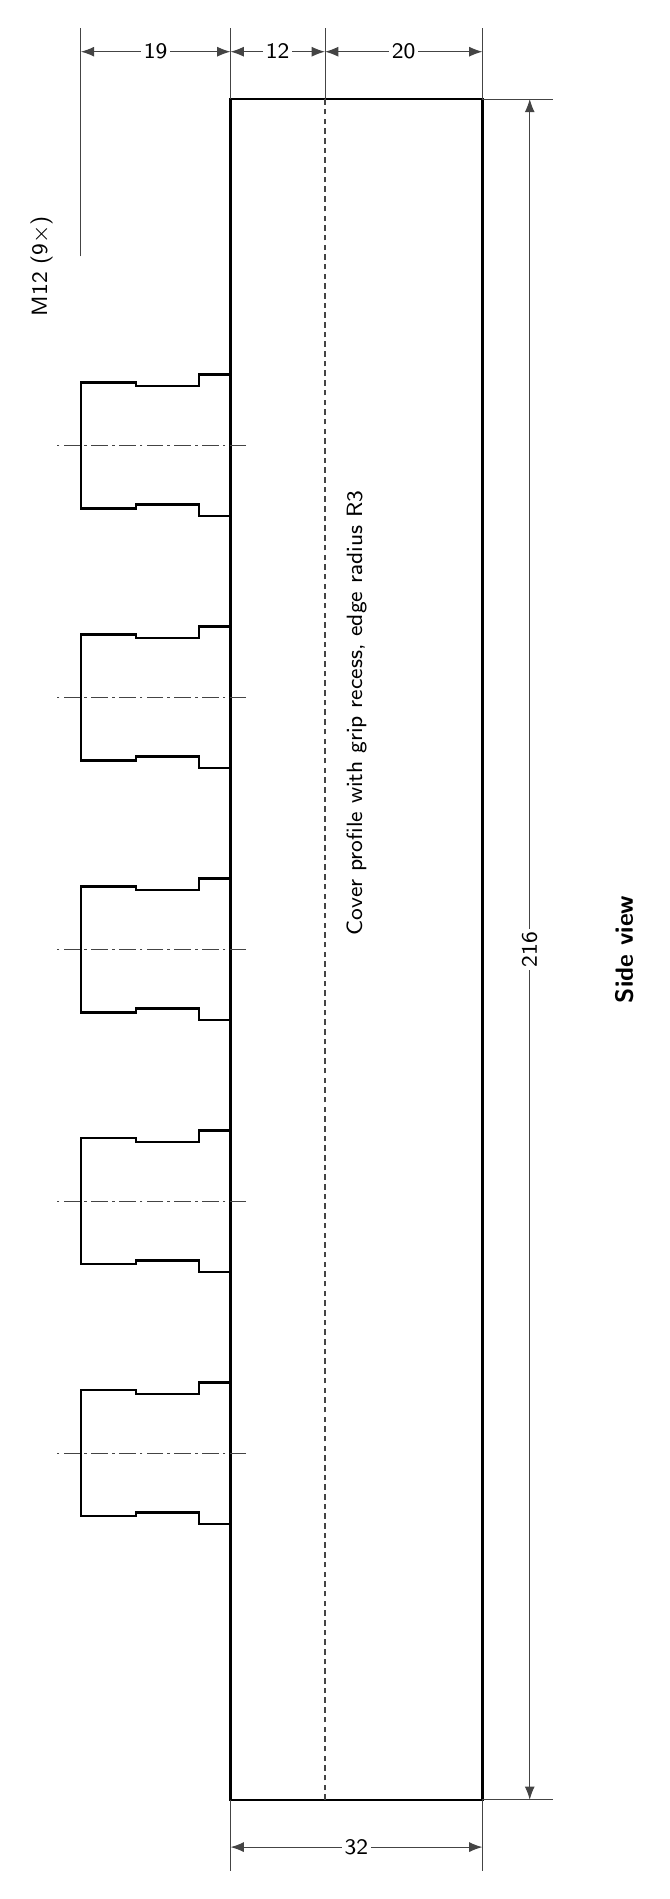
\begin{tikzpicture}[scale=0.1, rotate=90]
  % profile: base 20 + cover 12 = 32
  \draw[part] (-108,0) -- (108,0) -- (108,32) -- (-108,32) -- cycle;
  \draw[hidden] (-108,20) -- (108,20);
  % M12 connectors (protrusion 19: hex, threaded body, coupling ring)
  \foreach \x in {-64,-32,0,32,64}{
    \draw[part] (\x-9,32) -- (\x-9,36) -- (\x-7.5,36) -- (\x-7.5,44)
      -- (\x-8,44) -- (\x-8,51) -- (\x+8,51) -- (\x+8,44)
      -- (\x+7.5,44) -- (\x+7.5,36) -- (\x+9,36) -- (\x+9,32);
    \draw[center] (\x,30) -- (\x,54);
  }
  \node[dimtext, rotate=90, anchor=west] at (80,56) {M12 (9$\times$)};
  % height dimensions
  \draw[extline] (108,0) -- (117,0);
  \draw[extline] (108,20) -- (117,20);
  \draw[extline] (108,32) -- (117,32);
  \draw[extline] (88,51) -- (117,51);
  \draw[dimline] (114,0) -- (114,20) node[dimtext,midway]{20};
  \draw[dimline] (114,20) -- (114,32) node[dimtext,midway]{12};
  \draw[dimline] (114,32) -- (114,51) node[dimtext,midway]{19};
  \draw[extline] (-108,0) -- (-117,0);
  \draw[extline] (-108,32) -- (-117,32);
  \draw[dimline] (-114,0) -- (-114,32) node[dimtext,midway]{32};
  \draw[extline] (-108,0) -- (-108,-9);
  \draw[extline] (108,0) -- (108,-9);
  \draw[dimline] (-108,-6) -- (108,-6) node[dimtext,midway,rotate=90]{216};
  \node[dimtext, rotate=90] at (30,16) {Cover profile with grip recess, edge radius R3};
  \node[font=\small\bfseries, rotate=90] at (0,-18) {Side view};
\end{tikzpicture}
\end{center}

\newpage
\thispagestyle{fancy}
\begin{center}
{\small Sheet 4/4: isometric view of the compute module, connector side (not to scale)}
\end{center}
\vfill
\begin{center}
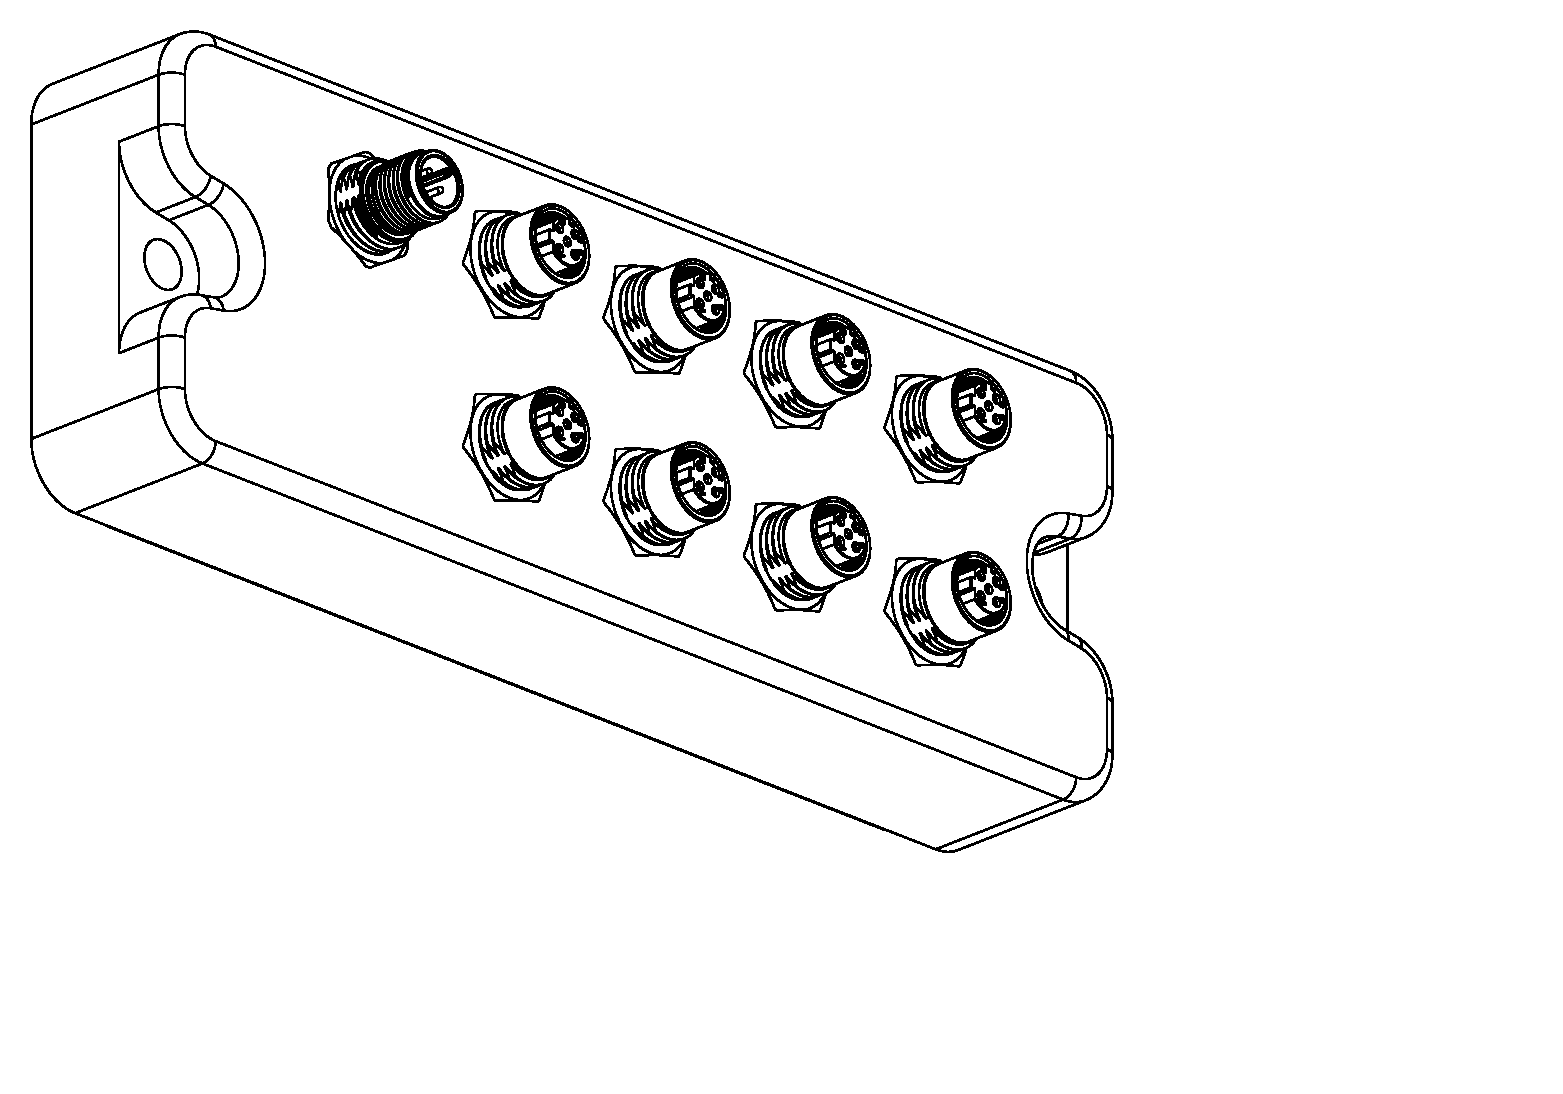
\includegraphics[width=0.95\textwidth]{horus-assembly.pdf}
\end{center}
\vfill
{\scriptsize All connectors M12, IP67: 8$\times$ D-coded (7$\times$ PoE LAN, 1$\times$ WAN, 4-pin Ethernet), pitch $32\times32$; 1$\times$ A-coded power-in (4-pin), rotated 45°. Cover fastening: 6$\times$ M3$\times$30. Subject to change without notice.}

\end{document}
